\section{Progress Log}
\begin{itemize}
    \item \textbf{October 10th:} At the project's inception, I made several considerations. I chose OpenGL over more extensive systems like Unity, prioritizing its lightweight nature, which is crucial in a project where frame rate and latency significantly impact user experience. My prior experience with OpenGL served as a valuable risk mitigation factor. To streamline development and avoid the hassle of building on multiple machines, I opted for Nix, a choice rooted partly in my familiarity with the software and my prior negative experience trying to build OpenGL applications of different machines. Nix's capability to ensure consistent builds with a single command across various machines appealed to me. As a proactive risk mitigation measure, I decided I should verify the feasibility/difficulty of building OpenGL within the Nix environment. My supervisor Nicole Simmons had access to Azure Kinects which would be a good camera option however they have a quite arbitrary package set which has not been packaged for nix yet as far as I was aware. I had experience using open source heading tracking for video games. It thought it might be good idea to investigate using a variation of aruco marker
          tracking in OpenCV with a webcam.

    \item \textbf{October 13th:} I attempted to implement an Aruco paper marker tracker using a Logitech C270 HD webcam, which proved unsuccessful. However I investigated the neural net tracking approach showed promise, but did not work that well  suggesting that upgrading to a higher-end webcam might yield better results.

    \item \textbf{October 19th:} I achieved a basic version of OpenGL building with Nix on my machine, initially utilizing some unsightly hardcoding, which I successfully refactored out.

    \item \textbf{October 22nd:} I established an automated development environment using Nix, which loads useful packages for building and debugging while configuring Visual Studio Code's intellisense to recognize the necessary libraries, simplifying development.

    \item \textbf{October 23rd:} I upgraded to a more recent version of OpenGL and eliminated hardcoded asset paths to ensure compatibility across various systems.

    \item \textbf{October 30th:} I deciced I would attempt to try and package Azure-Kinect-SDK in nix giving myself a 1 week cutoff, if I could not get it working by then I would switch to a different solution or ditch the idea of using nix altogether.

    \item \textbf{November 01st:} Progress continued as I managed to hack together an initial version of the Azure-Kinect-SDK on NixOS. However, reliability in the build process remained a concern. I had to fork the Azure-Kinect-SDK repository because it has officially been dropped by Microsoft and there are CMAKE build bugs on linux.

    \item \textbf{November 05th:} I managed to create a reliable build process by patching the RPATHs for the produced binaries using patchelf. Microsofts proprietary \texttt{libdepthengine.so} library that is used for sensing depth from the camera was clearly minimally patched to work on Ubuntu (the only "officially" supported unix based OS). To get it to work in Nix required patching out leftover redundant windows dll based paradigms which was very annoying.

    \item \textbf{November 06th:} I identified the need to address Git submodules' issues and build libk4a and k4atools separately. The Azure Kinect SDK used git submodules that don't work well with nix.

    \item \textbf{November 07th:} I resolved the GitHub submodules issue by employing Git fetch instead of including the flake in the repository. Additionally, I engaged in a productive meeting with my supervisor, Nicole, discussing the physical design of the "real world" versus the matrix, including a physical space mirroring "the matrix" dimensions, marked with Aruco cubes at each corner.

    \item \textbf{November 08th:} I split the Azure SDK flake into its dedicated GitHub repository, enabling it to build from there. Additionally, I created a separate package, libk4a, which k4a-tools (formerly known as k4aviewer) now utilizes. Although k4a-tools built successfully, I encountered challenges with libk4a due to missing dependencies.

    \item \textbf{November 13th:} I addressed the issue with libk4a not functioning by adding a specific dependency (udev) and refining code dependencies. I now stood theoretically prepared to commence development. I noted that the Kinect offered better field of view below than above for depth sensing.

    \item \textbf{November 23rd:} The day brought hours of troubleshooting a perplexing issue with the translation matrix, ultimately resolving it. Progress continued as I focused on familiarizing myself with OpenGL and working on achieving the room perspective.

    \item \textbf{November 25th:} I successfully simulated the virtual "room" behind the screen and embarked on exploring head tracking.

    \item \textbf{December 15th:} A Kinect Class was created, and basic frame reading functionality was implemented, paving the way for further exploration into eye tracking using OpenCV.

    \item \textbf{December 16th:} I drew inspiration from a student at cambridges masters thesis \cite{Zabarauskas2012} and devised a plan for obtaining eye position using a series of steps, including acquiring a raw RGB image from the Kinect, employing OpenCV for eye tracking, projecting onto depth data, and scaling for use as the viewer's position.

    \item \textbf{December 17th:} I achieved basic eye tracking using OpenCV and dlib, albeit with reduced speed due to CPU utilization. Further refinement and refactoring were required, drawing from insights gleaned from a relevant paper.

    \item \textbf{December 19th:} I successfully integrated CUDA support in OpenCV through my Nix build, despite encountering significant challenges. The next step was to create a pipeline for image compression to expedite recognition. Additionally, I made a GitHub issues page for maintaining a useful to-do list and performed an upgrade to the new NixOS 23.11 release while addressing issues related to building OpenCV with CUDA.

    \item \textbf{December 20th:} I accelerated dlib's performance significantly by utilizing CUDA image compression, acknowledging the trade-off between speed and resolution/accuracy. I contemplated the possibility of utilizing Mediapipe for facial recognition using GPU functions and considered optimizing face detection by selecting a smaller window based on prior head position.

    \item \textbf{December 29th:} After returning from a holiday, I resumed work on head tracking, resolving issues with camera coordinate alignment and making refinements to the code. I also addressed a concern related to paths being relative to the source directory rather than the Nix-store.

    \item \textbf{December 30th:} I resolved the local path issue and improved the readability of the Nix flake. My focus shifted towards model loading, currently utilizing TinyObjLoader.

    \item \textbf{December 31st:} I successfully achieved basic model loading, albeit with some complexities. I now loaded the Cornell box as the default scene, although textures remained a work in progress. Additionally, I streamlined the process of automatically downloading TinyObjLoader from GitHub.

    \item \textbf{January 02:} Progress continued with multithreading functionality and basic refactoring. My attention turned to 3D glasses, evaluating options like polarized 3D and Anaglyph 3D. I also explored reasons behind the slow face detection, attributing it primarily to the dlib face detector's performance. By enabling CUDA and AVX support, I managed to switch dlib to use a CNN which utilized the GPU, significantly improving performance. I had to fix a bug in the Nix package for dlib to enable GPU support because it wasn't actually using it.

    \item \textbf{January 03:} I faced challenges related to camera coordinates and perspective, leading to adjustments and continued exploration of rendering techniques. I recognized the importance of rendering to assess the 3D effect accurately and contemplated the possibility of establishing a proper test rig.

    \item \textbf{January 04:} The day brought further challenges in dealing with perspective issues, prompting a reversion to the original version of perspective. Additionally, I commenced work on loading textures onto models.

    \item \textbf{January 05:} Progress continued with the implementation of Blinn-Phong lighting and the start of downloading polyheavy models. A critical bug affecting perspective was identified and resolved.

    \item \textbf{January 06:} I achieved full model loading with face-by-face materials. I decided to use a chess set as a demonstration, as it offered an interesting perspective with its chequerboard pattern. The concept extended to the possibility of implementing hand interaction for playing chess against an AI opponent like Stockfish, which held significant potential as a captivating feature.

    \item \textbf{January 09:} In a significant development, I upstreamed my local fixes to the Dlib Nix package in a PR to nixpkgs, making them accessible to others.

    \item \textbf{January 10:} Started work on interim report.
\end{itemize}

\section{Current Status}
At the time of writing the interim report, I have achieved a working prototype that can display virtual 3D scenes to the viewer. The viewer can move their head around and see the scene from different perspectives. The render has been written from the ground up in OpenGL and is capable of rendering models loaded from OBJ files using the TinyObjLoader libary. The viewer's eye position is tracked using a Microsoft Azure Kinect. The render takes the live colour image stream from the Kinect compresses about 4 times on the GPU then uses a CNN in dlib to detect a face. With that face a 5 point facial landmark detector is run which gives up two points (the left and right side of the eye) we can use to use get an approximation for the position of the pupil. We then use the Kinect to map this point in camera space to the depth camera to get the 3D coordinates of the viewers eye. We then render the appropriate scene as can be seen in Fig~\ref{fig:prototype}.

\begin{figureBox}[label={fig:prototype}]{Current Working Prototype displaying a chessboard slightly extended out of the screen plane}
    \begin{minipage}[t]{0.48\textwidth}
        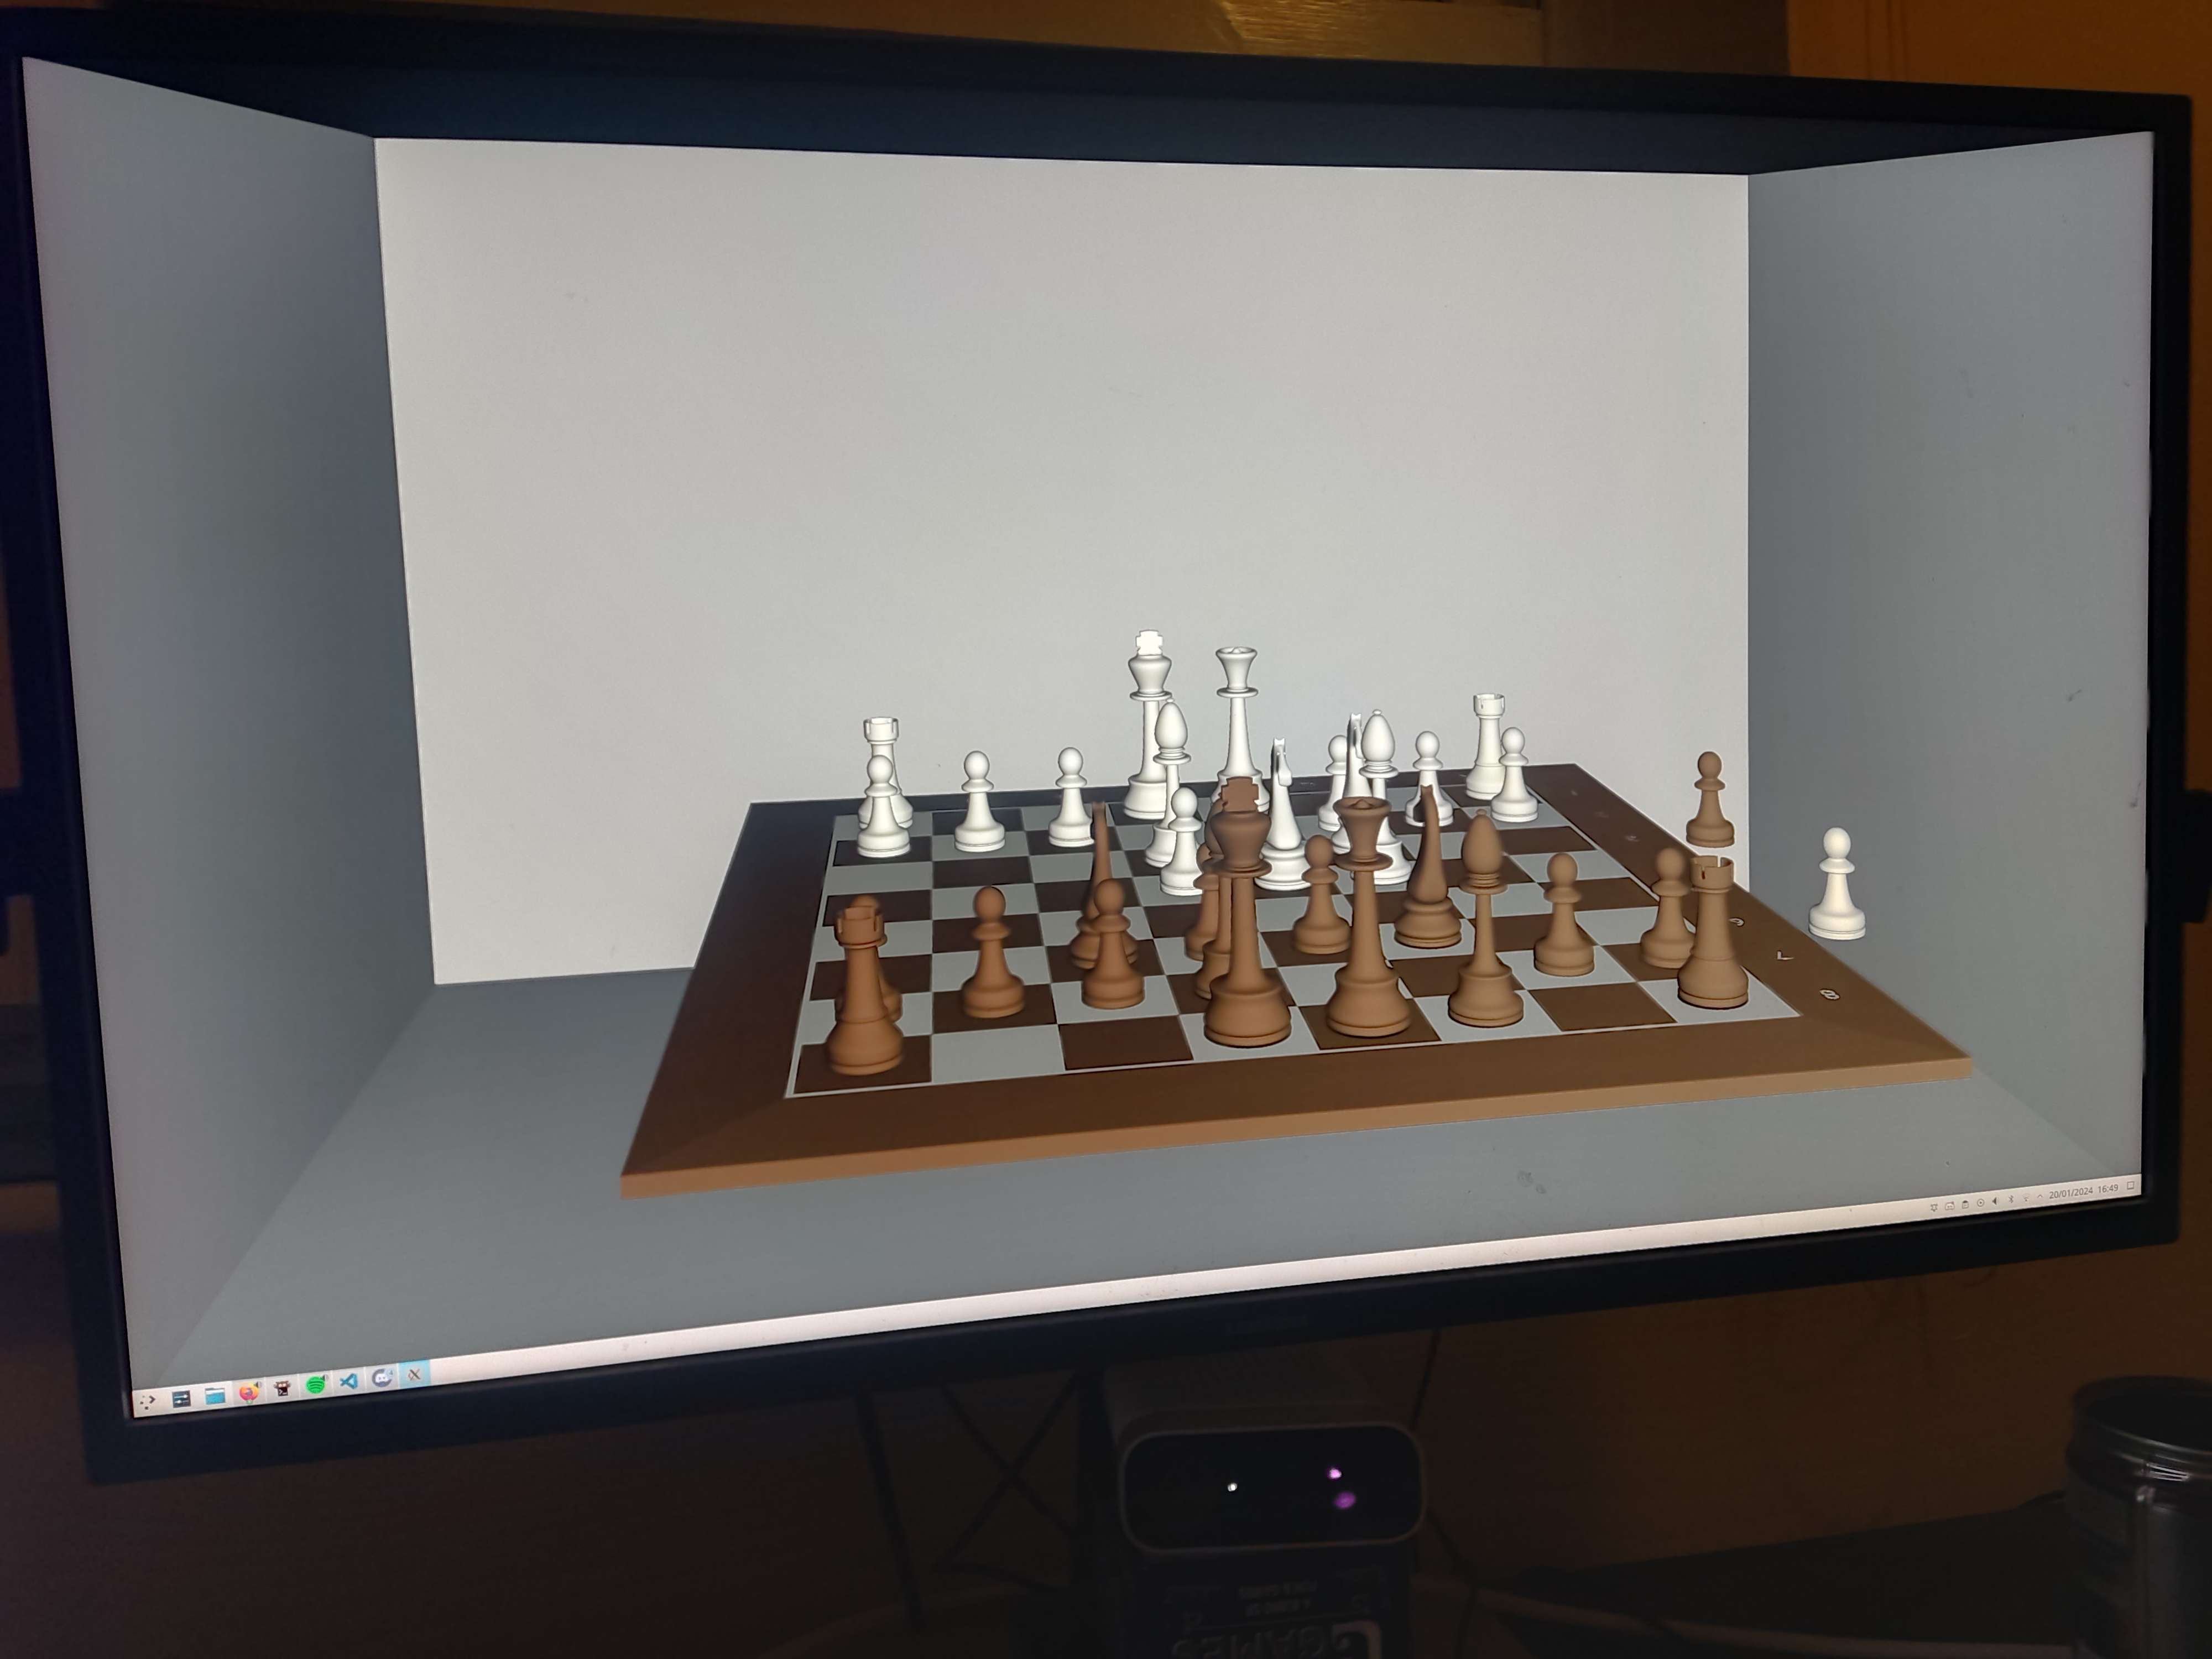
\includegraphics[width=\textwidth]{./project plan/figures/view_left.jpg}
        \small {a) View from the left.}
    \end{minipage}\hfill
    \begin{minipage}[t]{0.48\textwidth}
        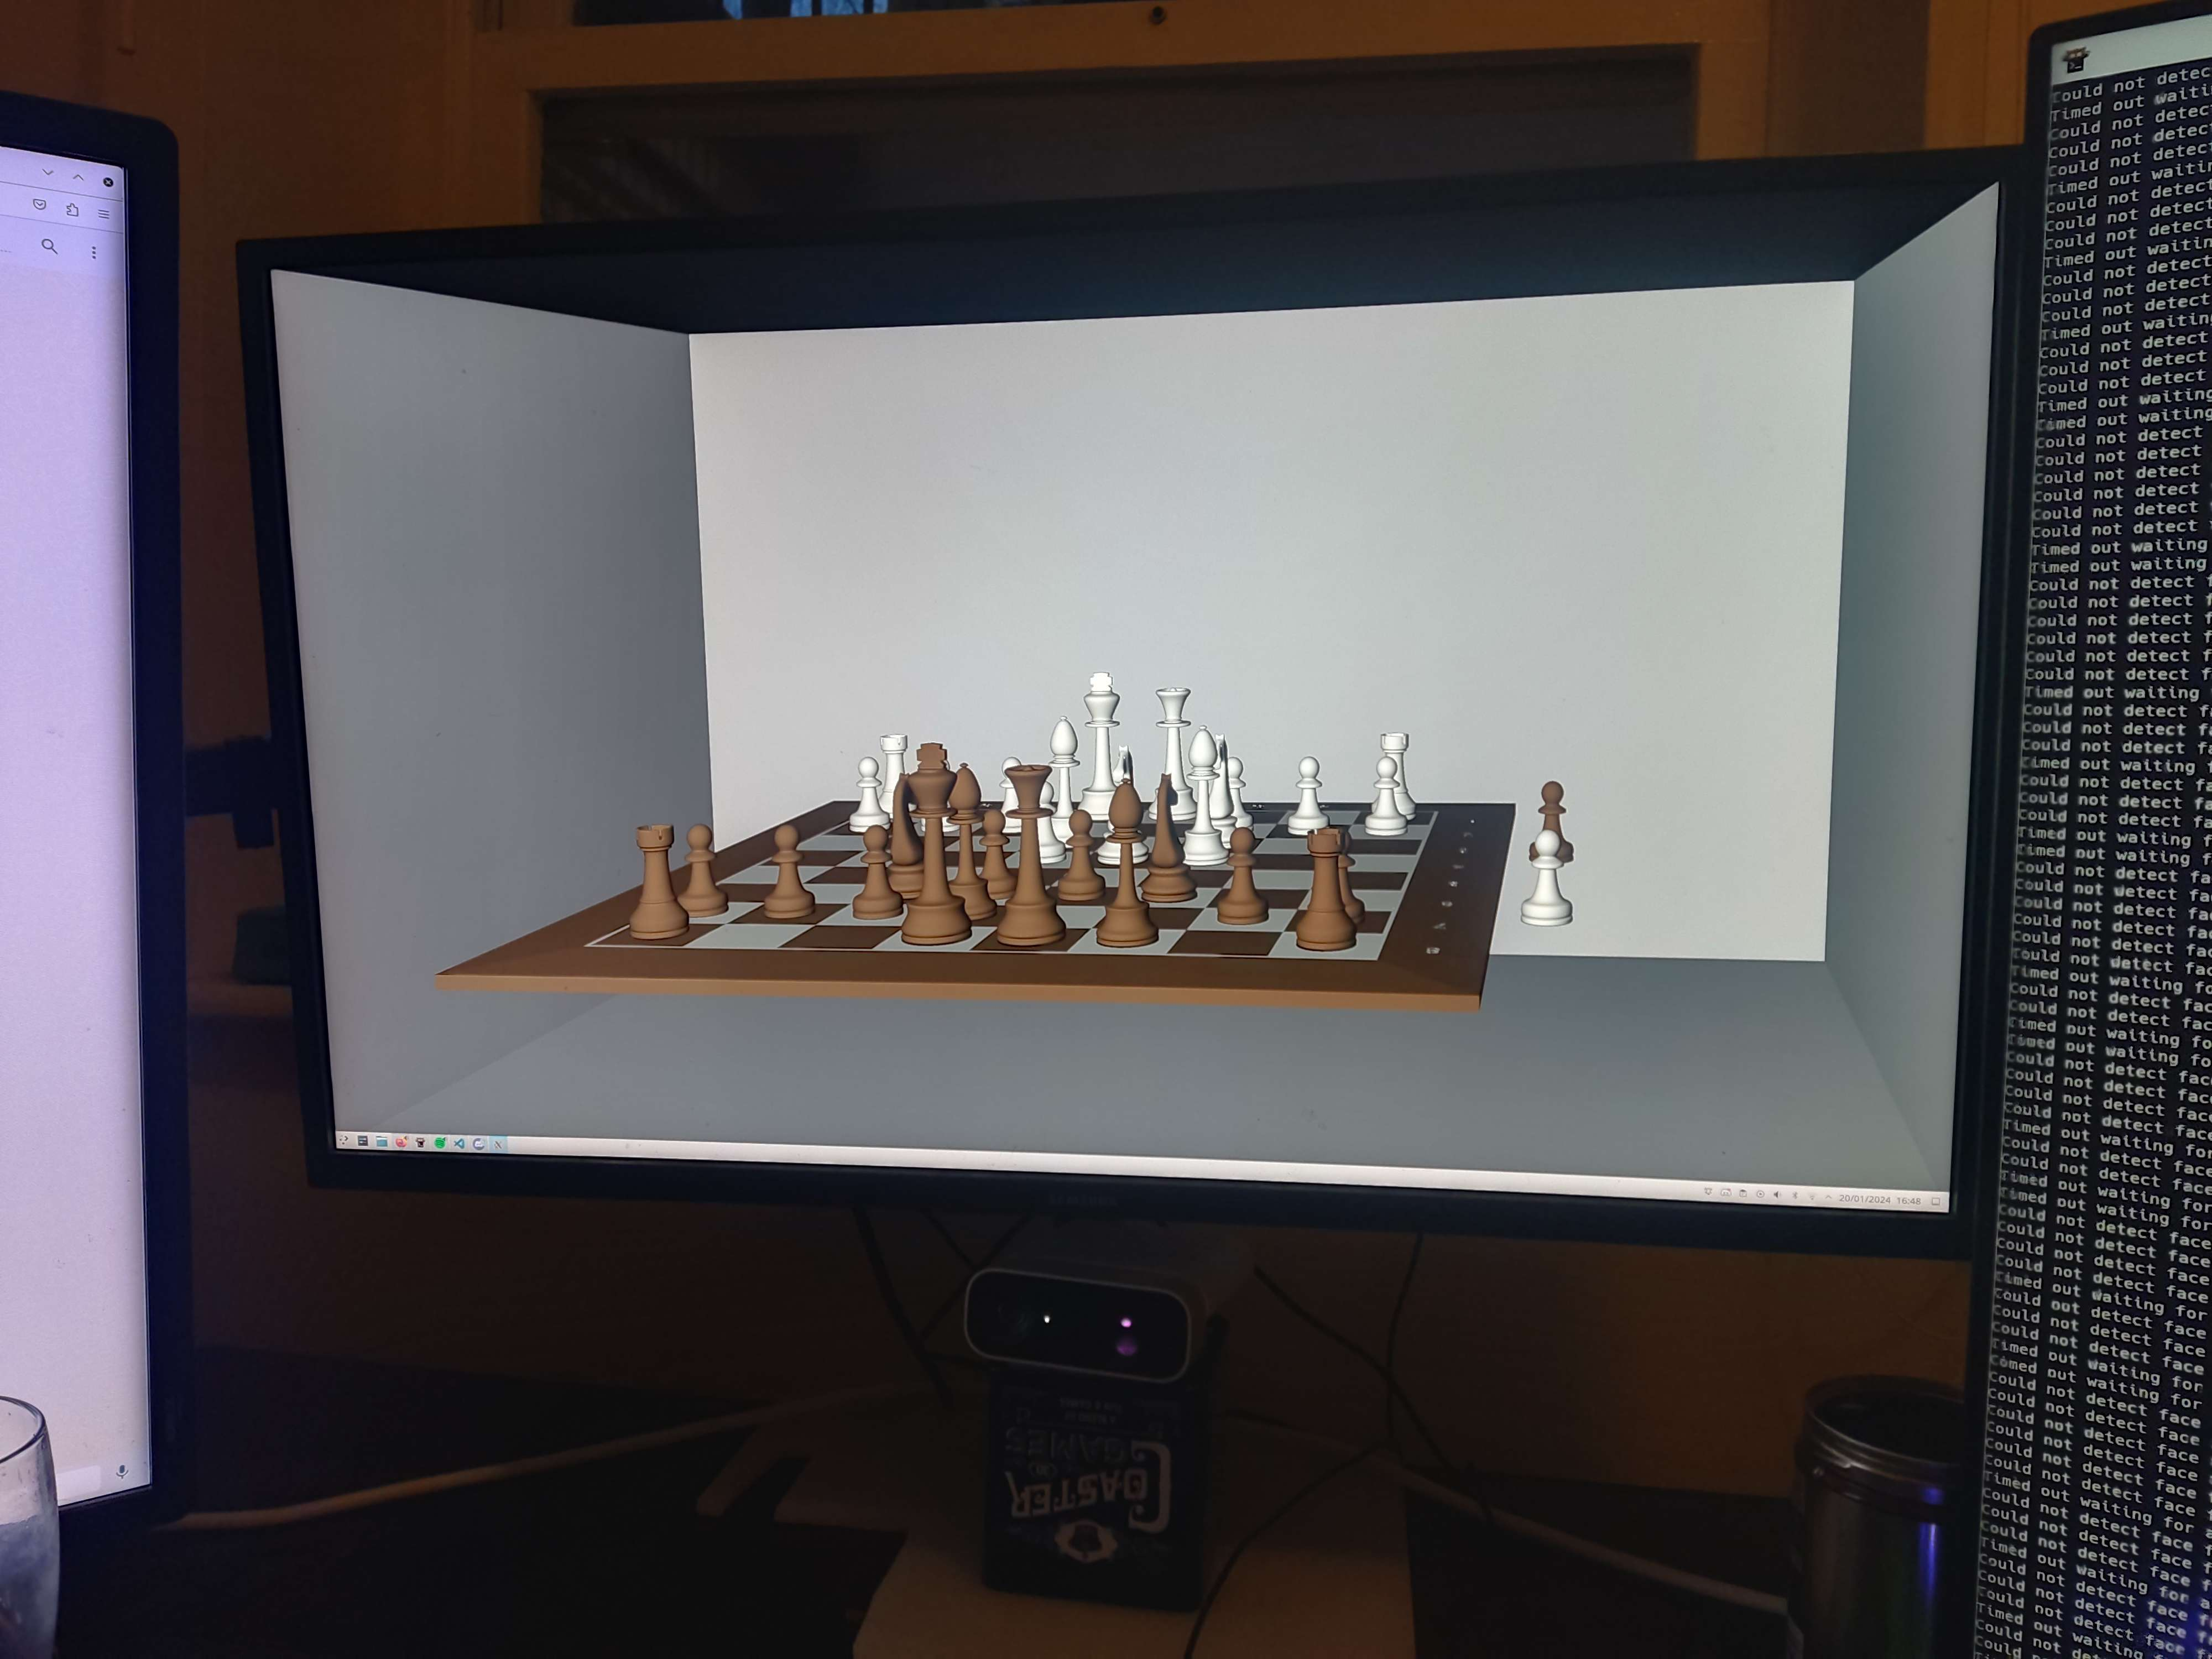
\includegraphics[width=\textwidth]{./project plan/figures/view_right.jpg}
        \small {b) View from the right.}
    \end{minipage}
\end{figureBox}

The repository is publically available at \url{https://github.com/RobbieBuxton/VolumetricSim} and is slightly over 1500 lines of C++ and nix code. The repository should (but not tested) be able to be run from any x86-intel machine with a nvidia gpu and azure kinect. All you need to do is install the nix package manager which I recommend downloading from here \url{https://zero-to-nix.com/concepts/nix-installer} and run 
\[\texttt{[shell:~]\$ sudo nix run github:RobbieBuxton/VolumetricSim}\]
 Nix will download and configure all dependencies, it will probably take a while on first run because we use CUDA and the nix community currently doesn't publically cache unfree software. \\

As a side effect of this project I have also created a repository of a package that will automatically build and run the Azure Kinect SDK on Nix. This is available at \url{https://github.com/RobbieBuxton/k4a-nix}. \\

This is a key milestone as represents the baseline functionality required to start the more interesting additions. This has de-risked the project as if some features turn out of be unfeasible it should not be difficult to pivot to a different approach while still having a significant deliverable.

\section{Future Milestones}
\subsection{Key milestones}
\begin{itemize}
    \item \textbf{Hand Tracking:} The next key milestone is to implement hand tracking. This will allow the user to interact with the virtual scene. I have not yet got a concrete idea about the best methods to do this yet but plan to organize a meeting with Andrew Davison to discuss this, as he is an expert in this field and hopefully should be able to point me in the right direction. I will be interested to find out if he thinks it is better to track in the point cloud or first on the colour camera and map to the point cloud. Furthermore, I predict this task will be the most difficult part of the project and could easily take a month or more.

    \item \textbf{Interactive Challenge:} To test the device we will need to create an interactive challenge. Not yet completely decided on what this will be yet, but I am leaning towards a chess game currently against an AI opponent. The user will be able to move the pieces with their hands and the AI will move its pieces using a chess engine. This will be a good test of the device as it will require the user to interact with the virtual scene and will be a good demonstration of the device's capabilities. I predict this task a week or two. This task is also completely dependent on the hand tracking challenge.

    \item \textbf{Shadows:} Shadows are a key part of giving the illusion of depth. I plan to implement shadows using ray tracing or shadow mapping. I have implemented ray tracing before in a previous project it worked well. However, I am not sure if it will be fast enough to run in real time. I will need to do some research into shadow mapping to see if it is a better option. I predict this task will take a week or less.

    \item \textbf{Calibration mode:} Currently the device is difficult to debug because the only method you have is if it looks correct. I am still not sure if it correctly calibrated, I.e if the screen is defined correctly in the basis of the camera and the offset is correctly measured. I plan to mode to verify if the simulator is calibrated correctly. I still need to do research to figure out the best way to do this. I predict this task will take a week or less.
    
    \item \textbf{Run User Study:} The final milestone is to run a user study to evaluate the device. I plan to run a user study with 10-20 participants. I will ask them to complete a questionnaire about their experience with the device and ask them to complete the interactive challenge. I predict this task will take a week or less. This will require ethics approval which I need to apply for after this interim report deadline.
\end{itemize}

\subsection{Optional milestones}
\begin{itemize}
    \item \textbf{Adapt to be compliant with OpenXR:} OpenXR is an open standard for virtual reality and augmented reality. It is supported by all the major players in the industry including Microsoft, Valve, Oculus, Google, and many more. It would be a good idea to adapt the project to be compliant with this standard, so it can load into any OpenXR compatible application. I am currently not sure how difficult this is or if it is even feasible.
 
    \item \textbf{Run on a Nvidia Jetson:} The nvidia jetson is a small embedded computer with a GPU. It would be interesting to see if the project could be adapted to run on this device. This would allow all the GPU heavy tasks to be on the device and you could plug the device into a monitor and have a portable volumetric display. The nvidia jetson is already packaged in nix so it would a function of fixing and bugs that from the new hardware and optimizing the code to run on a smaller gpu that my desktop which is am currently testing on. This would probably take a week or two. I already own a nvidia jetson.

    \item \textbf{Anaglyph 3D:} Anaglyph 3D is a method of displaying 3D images using filters typically red and green color filters and does not require special hardware. The 3D effect currently requires 1 eye to be closed so adding 3D support would make it a more immersive experience. I predict this task will take a day or two.
    
    \item \textbf{Realtime light detection:} Taking inspiration what I have learn from advanced graphics this term it might be interesting to add another camera, a fish eye lense and use that to generate a realtime light map. This would allow the virtual scene to be lit by the real world lighting. I have already talked to Prof Abhijeet Ghosh about this idea and he thinks it is feasible. However this is going in a slightly different direction with the project. I predict this task will take a week or two.
    
    \item \textbf{Improve compatibility:} Currently the project only works on nvidia GPUs. It would be good to improve compatibility to work on AMD GPUs and Intel GPUs and also run without a GPU. It was also be good to support different depth cameras other than the Kinect as this has been discontinued by Microsoft. This would require a lot of refactorings and would probably take a week or two.
    
    \item \textbf{Tracker Logging:} It would be good to log the tracker data to a file so that it can be replayed later. This would allow experiments to be reproduced without having to use the device and would allow people to externally verify experiments. This would require a lot of refactorings and would probably take a week or two.
\end{itemize}